\documentclass[11pt,a4paper]{article}
\usepackage[utf8]{inputenc}
\usepackage{amsmath, amssymb, amsthm}
\usepackage{geometry}
\usepackage{graphicx} % Include graphics
\usepackage{hyperref} % Hyperlinks
\usepackage{enumerate} % Customizable enumeration
\geometry{a4paper, margin=1in}

% Theorem Environments - Section numbering included
\theoremstyle{plain}
\newtheorem{theorem}{Theorem}[section]
\newtheorem{lemma}[theorem]{Lemma}
\newtheorem{proposition}[theorem]{Proposition}
\newtheorem{corollary}[theorem]{Corollary}
\theoremstyle{definition}
\newtheorem{definition}[theorem]{Definition}
\newtheorem{example}[theorem]{Example}
\newtheorem*{definition*}{Definition}
\theoremstyle{remark}
\newtheorem*{remark}{Remark}
\newtheorem*{note}{Note}

\begin{document}

% \tableofcontents

\pagebreak

\section{Setup}

\subsection{Why use Sobolev Spaces?}

In theoretical investigations of the degree of approximation, one typically makes an a priori assumption that the target function \(f\) , although itself unknown, belongs to some known class of functions. In this report, we are interested in the Sobolev classes.
By use of sobolev spaces we can leverage more information than just input-output data pairs. By assuming our target function belongs to some smoothness class, we can use this information to improve the performance of our neural networks. This can be taken advantage of in the training process, where we have seen Sobolev training in action already in the literature. \cite{enwiki:1223692835}. We first attempt to instead use architecture to leverage this information, and see if we can improve the performance of our neural networks. We must begin by understanding the existing results in the literature, and then attempt to translate these results into a practical framework, to see if these results hold true in practice.

This section focuses on the results from Poggio, T. and Liao, Q. (2018) 'Theory I: Deep networks and the curse of dimensionality', Bulletin of the Polish Academy of Sciences: Technical Sciences, 66(6). doi: 10.24425/bpas.2018.125924. Within this paper, the authors state two theorems, which are as follows:

\begin{enumerate}
    
\item \textbf{Theorem 1}: (Shallow Networks)

It states that for a function \( f \in W_{m}^{n} \), the set of all functions of \(n\) variables with continuous partial derivatives up to order \(m < \infty \) such that \(\left\lVert f\right\rVert + \sum_{1\leq \left\vert \mathbf{k}  \right\vert_{1} \leq m} \left\lVert \mathbf{D}^{k} f\right\rVert \leq 1  \), and an activation function \( \sigma: \mathbb{R} \rightarrow \mathbb{R} \) that is infinitely differentiable and not a polynomial, the complexity of shallow networks that provide accuracy at least \( \varepsilon \) is 
\[ N = O(\varepsilon^{-n/m}) \]

\item \textbf{Theorem 2}: (Deep Networks)

It considers a function \( f \in W_{m}^{2,n} \), the class of all compositional functions \(f\) of \(n\) variables with a binary tree architecture and constituent functions \(h\)  in \(W_{m}^{2}\)  and a deep network with a compositional architecture.\\
The activation function \( \sigma: \mathbb{R} \rightarrow \mathbb{R} \) in this context is also infinitely differentiable and not a polynomial. The complexity of the network necessary to provide an approximation with accuracy at least \( \varepsilon \) is 

\[ N = O((n - 1)\varepsilon^{-2/m}) \]
\end{enumerate}

Theorem 1 is already a classic result, with Theorem 2 being the new result, which we pay particular attention to later in this report.

% Insert diagram of deep network
\begin{figure}
    \centering
    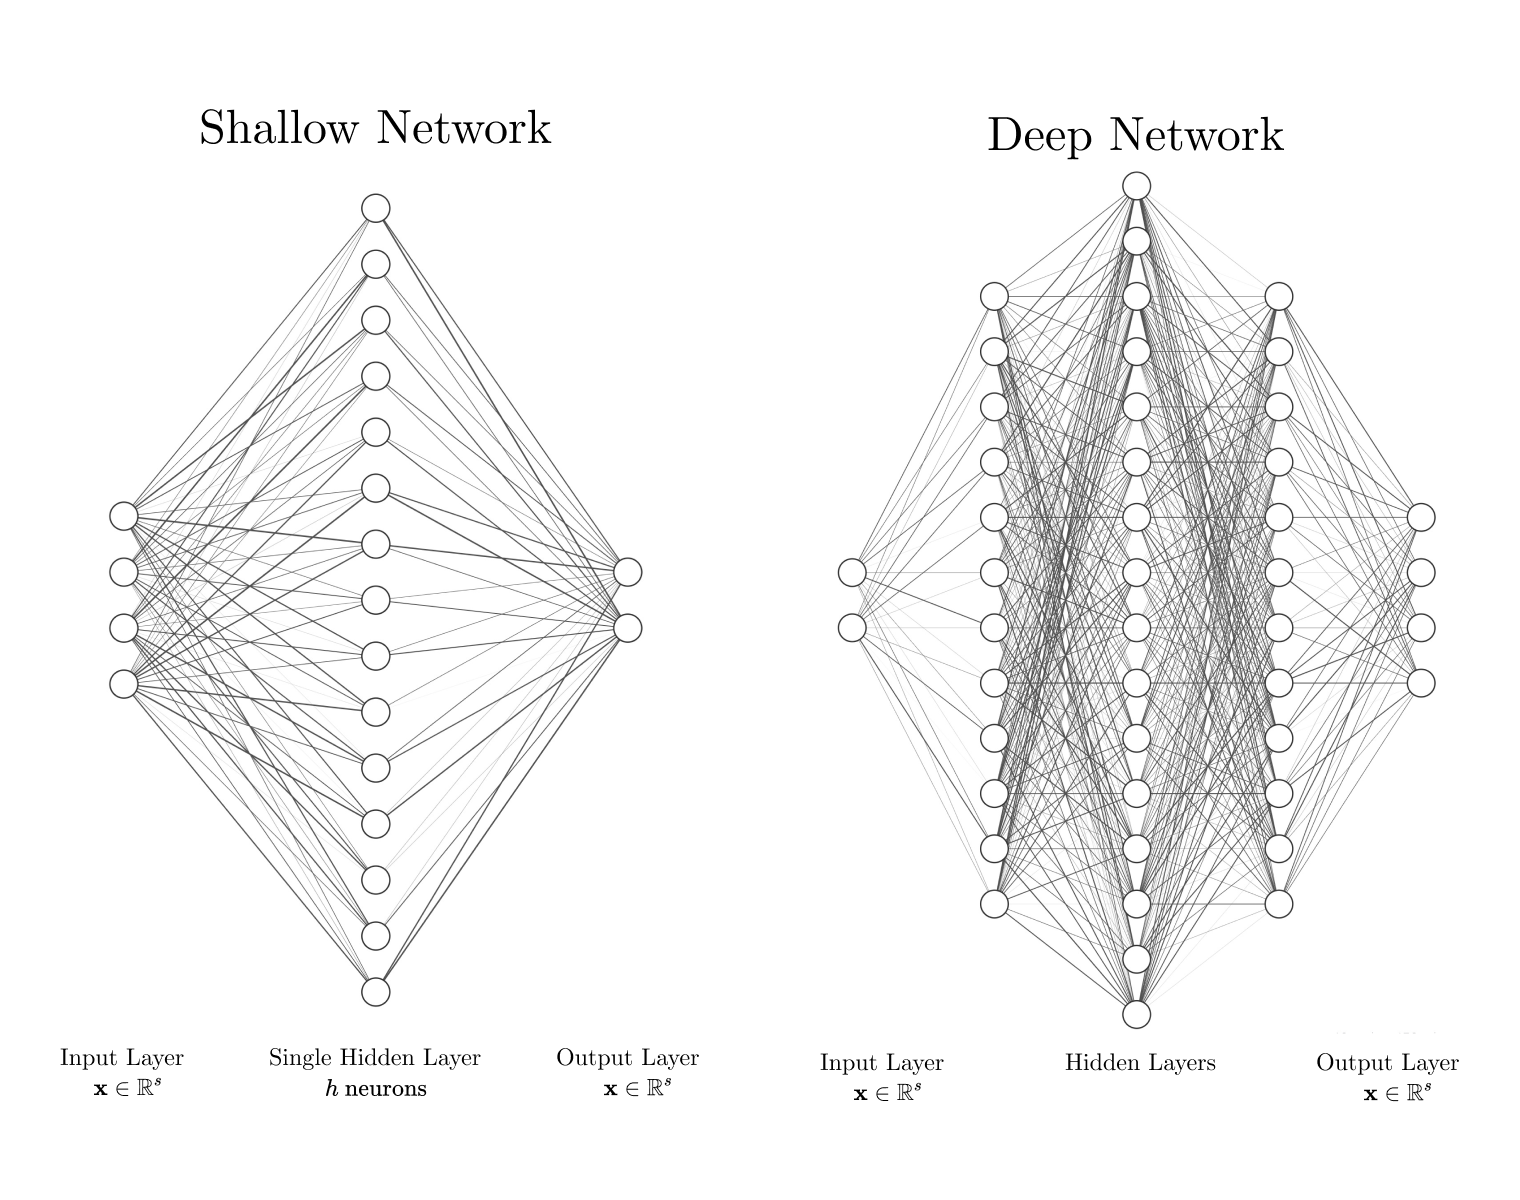
\includegraphics[width=0.8\textwidth]{diags/shallow_deep.png}
    \caption{Shallow and Deep Neural Network}
\end{figure}



\begin{definition}[Shallow Neural Network (Single Hidden Layer)]

A shallow neural network with a single hidden layer is defined by the following components:

\begin{itemize}
  \item \textbf{Input Layer:} Let \(\mathbf{x} = (x_1, x_2, \ldots, x_d)^T\) represent the input vector where \(d\) denotes the number of input features, thus \(\mathbf{x} \in \mathbb{R}^d\).

  \item \textbf{Hidden Layer:} The hidden layer consists of \(h\) neurons. Each neuron \(j\) applies a transformation to the input vector, characterized by a weight vector \(\mathbf{w}_j \in \mathbb{R}^d\) and a scalar bias \(b_j\). The activation function \(\sigma\) is applied to the linear combination of the inputs:
    \[
    z_j = \sigma(\mathbf{w}_j^T \mathbf{x} + b_j)
    \]
    The output of the hidden layer can be expressed as \(\mathbf{z} = (z_1, z_2, \ldots, z_h)^T \in \mathbb{R}^h\).

  \item \textbf{Output Layer:} Assuming a single output neuron, the final output \(y\) of the network is produced by applying another activation function \(\phi\) to the linear combination of the hidden layer outputs:
    \[
    y = \phi(\mathbf{v}^T \mathbf{z} + c)
    \]
    where \(\mathbf{v} \in \mathbb{R}^h\) and \(c\) is a scalar bias.
\end{itemize}

\begin{definition}[Deep Neural Network (Multiple Hidden Layers)]

A deep neural network is an extension of a shallow network that includes multiple hidden layers. Let there be \(L\) hidden layers, each capable of transforming its input into a higher-level representation:

\begin{itemize}
    \item \textbf{Input Layer:} Similar to the shallow network, \(\mathbf{x} \in \mathbb{R}^d\).
    
    \item \textbf{Hidden Layer}  For each layer \(i\) from 1 to \(L\), let \(\mathbf{z}_i\) denote the output of layer \(i\), with \(\mathbf{z}_i \in \mathbb{R}^{h_i}\) where \(h_i\) is the number of neurons in layer \(i\). The transformation in layer \(i\) is defined as:
    \[
    \mathbf{z}_i = \sigma_i(\mathbf{W}_i \mathbf{z}_{i-1} + \mathbf{b}_i)
    \]
    Here, \(\mathbf{W}_i \in \mathbb{R}^{h_i \times h_{i-1}}\) represents the weight matrix, \(\mathbf{b}_i \in \mathbb{R}^{h_i}\) the bias vector, and \(\sigma_i\) the activation function, with \(\mathbf{z}_0 = \mathbf{x}\) as the initial input.

    \item \textbf{Output Layer:} The network output \(y\) is given by:
  \[
  y = \phi(\mathbf{v}^T \mathbf{z}_L + c)
  \]
  where \(\mathbf{v} \in \mathbb{R}^{h_L}\) and \(c\) is a scalar bias. The function \(\phi\) here denotes the activation function used at the output.

These structures enable the modeling of functions of varying complexity and are commonly used in tasks ranging from regression to classification.
We can further describe more complicated architectures of deep networks using directed acyclic graphs (DAGs). With each of the nodes in the graph representing a function, and each of the edges representing a composition, we can represent a wide range of functions. We will more carefully define this later.

\end{itemize}

\subsection{Norms}
We first take care to mention the norms we are using. If we intend to measure the quality of an approximation, we must carefully consider how to do this and how the use of various norms interact with one another, and what that implicates for our results. In particular we use 2 types of norms.

\subsubsection{The \( L^p \)-norm (\( \|\cdot\|_p \))}

This norm is used to measure the approximation error between the function \( f \) and the sum involving the function \( \phi \) and coefficients \( a_j(f) \) - the neural network.

We use \(\Pi_{\phi ; n,s}\) to denote the set all neural networks with \(n\) neurons, each evaluating the activation function \(\phi \) for a function of \(s\) variables.

If \( A \subseteq R^{s}\) is Lebesgue measurable, and \(f : A \to R\) is a measurable function, we define the \(L^{p} (A)\) norms of \(f\) as follows:   
   \[
   \|f\|_{p,A} = 
   \begin{cases} 
   \left( \int_{A} |f(x)|^p dx \right)^{1/p}, & \text{for } 1 \leq p < \infty, \\
   \text{ess sup}_{x \in A} |f(x)|, & \text{for } p = \infty.
   \end{cases}
   \]


   The class of all functions such that \(\left\lVert f\right\rVert_{p,A} < \infty \) is denoted by \(L^p(A)\) 

   Take \(L^{\infty }(A)\) as the space of continuous functions on \(A\).

   Throughout this report we take \(A = [-1,1]^s\), unless explicitly stated otherwise.

   This norm is used in the inequality:

   \[ \left\|f - \sum_{j=1}^{n} a_j(f) \phi(A_j(\cdot) + b)\right\|_p \leq c n^{-r/s} \|f\|_{W^p_{r,s}} \]

   where it measures the difference between the function \( f \) and its approximation.

   We measure the \textit{degree of approximation} of \(f\) by the expression

   \[
    E_{\phi;n,p} = \inf\{ \left\| f - g \right\|_p : g \in \Pi_{\phi ; n,s} \}
   \]

   The quantity \(E_{\phi ; n,p}\)  denotes the theoretically minimal error that can be achieved in approximating the function \(f\)  in the \(L^p\)  norm by generalized translation networks with \(n\)  neurons each evaluating the activation function \(\phi \) 

\subsubsection{Sobolev Norm \((\|\cdot\|_{W^p_{r,s}})\) }

We first define the space as follows: 

Let \(r \geq 1\) an integer and \(Q\) a cube in \(\mathbb{R}^{s}\). The class \(W^p_{r,s}(Q)\) consists of all functions with \(r - 1\) continuous partial derivatives on \(Q\) which in turn can be expressed (almost everywhere on \(Q\)) as indefinite integrals of functions in \(L^p(Q)\). Alternatively, the class \(W^p_{r,s}(Q)\) consists of functions which have, at almost all points of \(Q\), all partial derivatives up to order \(r\) such that all of these derivatives are in \(L^p(Q)\). 

The Sobolev norm of \(f \in W^p_{r,s}(Q)\) is defined by 

\[
\|f\|_{W^p_{r,s}(Q)} = \sum_{0\leq |k| \leq r}  \left\lVert D^{\mathbf{k}} f\right\rVert_{p,Q}   
\]

where for the multi-integer \( \mathbf{k}  = (k_1,...,k_s) \in \mathbb{Z}^s \), \( 0 \leq \mathbf{k}  \leq r \) means that each component of \( \mathbf{k}  \) is nonnegative and does not exceed \( r \), \( |\mathbf{k} | := \sum_{j=1}^{s} |k_j| \) and 

\[
    D^{\mathbf{k} }f = \frac{\partial^{|\mathbf{k} |} f}{\partial x_1^{k_1} \cdots \partial x_s^{k_s}}, \quad k \geq 0
\]

Again \(W^{\infty }_{r,s}(Q)\) will denote the class of functions which have continuous derivatives of order \(r\) and lower. As before, if \(Q = [-1, 1]^s\), we will not mention it in the notation. Thus, we write \(W^p_{r,s} = W^p_{r,s}([-1, 1]^s)\) etc.

Since the target function itself is unknown, the quantity of interest is
\[
    E_{\phi ; n,p,r,s} := \sup\{E_{\phi ; n,p}(f) : \|f\|_{W^p_{r,s}} \leq 1\}
\]

Here we take the fact that that any function in \(W^p_{r,s}\) can be normalized so that \( \|f\|_{W^p_{r,s}} \leq 1 \). So our quantity \(E_{\phi ; n,p,r,s}\) is the maximal error that can be achieved in approximating functions in \(W^p_{r,s}\) by generalized translation networks with \(n\) neurons each evaluating the activation function \(\phi \), with the assumption that the target function \(f \in W^p_{r,s}\) is properly normalised.



\subsection{Classical results}

We first refer to the universal approximation theorem, which states that neural networks with a single hidden layer can approximate any function that is continuous and bounded, up to a constant. This is a fundamental result in the field of neural networks, and is widely used in the literature. \cite{goodfellow2016deep}.
From the universal approximation theorem, we know that both shallow and deep networks can approximate arbitrarily well any function of \(n\) variables on a compact domain. In particular, we can make the following statement.

\subsubsection{Theorem 1: Approximation by Shallow Networks}

Let \(1 \leq d \leq s\), \(r \geq 1\), \(n \geq 1\) be integers and \(1 \leq p \leq \infty\). Let \(\phi: \mathbb{R}^d \rightarrow \mathbb{R}\) be infinitely many times continuously differentiable in some open sphere in \(\mathbb{R}^d\). Here we also denote the space of shallow networks by \(\Pi_{\phi ; n,s}\), for some fixed \(n\). It is further assumed that there exists a point \(b\) in this sphere such that

\begin{equation}
    D^k \phi(b) \neq 0, \mathbf{k} \in \mathbb{Z}^d, \mathbf{k} \geq 0
\end{equation}

Then, there exist \(d \times s\) matrices \(\{A_j\}_{j=1}^n\) with the following property: For any function \(f\) in the Sobolev space \(W^p_{r,s}\), there exist coefficients \(a_j(f)\) such that

\[ \left\| f - \sum_{j=1}^{n} a_j(f) \phi(A_j(\cdot) + b_{j}) \right\|_p \leq c n^{-r/s} \|f\|_{W^{p}_{r,s}} \]

Here, the functionals \(a_j\) are continuous linear functionals on \(W^p_{r,s}\).

In particular, 

\[ E_{\phi;n,r,s,p} \leq c n^{-r/s} \]

where \( E_{\phi;n,r,s,p} \) denotes the maximal error that can be achieved in approximating functions in \(W^p_{r,s}\) by generalized translation networks with \(n\) neurons each evaluating the activation function \(\phi \), with the assumption that the target function \(f \in W^p_{r,s}\) is properly normalised.

\subsubsection{Proof of Theorem 1}

% In this subsection the numbers of propositions and equations will correspond to those in the Mhaskar paper.

\paragraph{Useful definitions and clarifications} 

\begin{enumerate}
    \item \(W^{p}_{r,s} (Q)\) - the Sobolev space of all functions that have at almost all points in \(Q\), all partial derivatives up to order \(r\) and all of these derivatives are in \(L^p(Q)\). With \(s\) the number of dimensions.
    \item \(\left\vert \mathbf{k}  \right\vert = \sum_{j} k_{j}\)
    \item  \(0 \leq \mathbf{k} \leq \mathbf{r}  \iff 0 \leq k_{j}\leq r_{j} \forall j\) 
    \item \(L^{p^{\ast} } := L^{p}([-\pi ,\pi ]^s) \), \(W^{p^{\ast} }_{r,s} := W^{p}_{r,s} ([-\pi ,\pi ]^s)\) 

    \item[(\textbf{eq.} 3.1)] \textbf{Fourier Coefficients}: For a function \( g \in L^{p^*} = L^{p}([-\pi ,\pi ]^s) \), its Fourier coefficients are given by the following, where \( \mathbf{k} \) is a multi-index in \( \mathbb{Z}^s \), and \( \mathbf{t}  \) is in the domain \( [-\pi, \pi]^s \).

    \[
      \hat{g}(\mathbf{k}) := \frac{1}{(2\pi)^s} \int_{[-\pi,\pi]^s} g(t)e^{-i \mathbf{kt}} d \mathbf{t}, \quad \mathbf{k} \in \mathbb{Z}^s.  
    \]


    \item[(\textbf{eq.} 3.2)]\textbf{Partial Sums of the Fourier Series}: The partial sum \( s_m(g, t) \) of the Fourier series of \( g \) is given as follows, where we denote \(\mathbf{k} \leq \mathbf{m} \) if \(k_{j} \leq m_{j}\) for \( 1 \leq  j \leq s\) 
    
    \[
        s_m(g,t) := \sum_{-\mathbf{m} \leq \mathbf{k} < \mathbf{m}} \hat{g}(k)e^{i \mathbf{kt}}, \quad \mathbf{m}  \in \mathbb{Z}^s, \quad \mathbf{m}  \geq 0, \quad \mathbf{t} \in [-\pi, \pi]^s,
    \]

    \item[(\textbf{eq.} 3.3)]\textbf{de la Vallée Poussin Operator}: The de la Vallée Poussin operator \( v_n(g, t) \) for a function \( g \) is defined as the average of the partial sums \( s_m(g, t) \) where \( m \) ranges from \( n \) to \( 2n \). This operator is used to create a smoothed approximation of the function \( g \).
    
    \[
        v_n(g,\mathbf{t} ) := \frac{1}{(n+1)^s} \sum_{n \leq \mathbf{m} \leq 2n} s_{\mathbf{m}}(g,t), \quad n \in \mathbb{Z}, \quad n \geq 0, \quad \mathbf{t} \in [-\pi, \pi]^s,
    \]


\end{enumerate}

\paragraph{Idea for the Proof}

For every integer \(m \geq r, \exists \) polynomial \(P_{m}(f)\) of coordinatewise degree not exceeding \(m\) such that \(\forall f \in W^{p}_{r,s}\) 
\[
\|f - P_{m}(f)\|_{p,[-\pi,\pi]^s} \leq \frac{c}{m^r} \|f\|_{W^{p*}_{r,s}}  
\]

Aim to express each monomial in \(P_{m}(f)\) with suitable derivative of \(\phi \), then take each derivative approximations and approximate it by an appropriate divided difference method involving \(O(m^s)\) evaluations of \(\phi \) 


\paragraph[]{Proposition 3.1 Statement}

([insert ref here])

\begin{itemize}
    \item  Given integers \( r \geq 1 \), \( s \), \( m \geq 1 \), and \( 1 \leq p \leq \infty \).
    \item  Let \( g \) be a function in the Sobolev space \( W^{p^{\ast}}_{r,s} \).
    
    \item Then \( v_m(g) \) is defined as a trigonometric polynomial of coordinate-wise order at most \( 2m \). This means that \( v_m(g) \) is a polynomial composed of sine and cosine terms, where the highest frequency term has a frequency of \( 2m \).
    
    Here \( v_m(g) \) is defined as the de la Vallée Poussin operator applied to \( g \), we omit the \(t\) dependence for brevity.
    \item And 
    \setcounter{equation}{1} 
    \begin{equation}
        \|g - v_m(g)\|_{p, [-\pi, \pi]^s} \leq \frac{c}{m^r} \|g\|_{W^{p*}_{r,s}}
    \end{equation}
    \item further,
    \begin{equation}
        \sum_{0 \leq \mathbf{k} < 2m} |\Hat{v_m(g)}(\mathbf{k})| \leq cm^\alpha \|g\|_{W^{p*}_{r,s}}  \quad \text{where} \quad \alpha = \frac{s}{\min(p,2)} 
    \end{equation}
\end{itemize}

\paragraph*{Key Result (Inequality 3.4)}

\begin{itemize}
    \item  The proposition states that the \( L_p \) norm of the difference between \( g \) and its trigonometric polynomial approximation \( v_m(g) \) is bounded. Specifically:

    \setcounter{equation}{1} 
    \begin{equation}
        \left\|g - v_m(g)\right\|_{p, [-\pi,\pi]^s} \leq \frac{c}{m^r} \|g\|_{W^r_{p, s}^*}
    \end{equation}

    \item  Here, \( \|g - v_m(g)\|_{p, [-\pi,\pi]^s} \) represents the \( L_p \) norm of the error (or the difference) between the function \( g \) and its approximation \( v_m(g) \) over the \( s \)-dimensional cube \( [-\pi, \pi]^s \).
    \item \( c \) is a constant that depends on \( p \), \( r \), \( s \), and possibly other factors, but not on \( m \) or \( g \).
\end{itemize}

The idea follows to make a periodic function from a function on \([-1,1]^s\). The standard way to achieve this is via a cosine substitution; \(x_{j} = \cos (t_{j}) 1 \leq j \leq s, \mathbf{x} \in [-1,1]^s, \mathbf{t} \in [-\pi ,\pi ]^s\). This substitution doesn't work as the \(L^p\) norms are no longer equal under this substitution.\\

Instead construct the following.\\
We first have from [insert ref] that there exists a continuous linear operator \( T: W_{r,s}^{p} \to W_{r,s}^{p}([-2,2]^s) \) such that the restriction of \( T(f) \) on \( [-1,1]^s \) is (almost everywhere) equal to \( f \). The continuity of the operator \( T \) means that
\[
    \|T(f)\|_{W_{r,s}^{p}([-2,2]^s)} \leq c \|f\|_{W_{r,s}^{p}}  
\]
for every \(f \in W_{r,s}^{p}\), This means that the operator \( T \) maps a function in the Sobolev space \( W_{r,s}^{p} \) to a function in the same space but defined on a larger domain, \( [-2, 2]^s \), we construct this operator later.

If we find in practice we have an \(f\) already appropriately defined on \([-2,2]^s\), then we can simply work with \(f\) itself rather than \(T(f)\), however our bounds would then depend on the respective Sobolev space; \(W_{r,s}^{p}([-2,2]^s)\) \\

We now define \(\psi \) be an infinitely differentiable function that takes the value 1 on \([-1,1]^s\) and \(0\)  outside the interval \([-3/2,3/2]^s\). Then the function \(T(f)\psi \) coincides with \(f\) on \([-1,1]^s\) and is identically zero outside \([-3/2,3/2]^s\) and

\setcounter{equation}{3} 
\begin{equation}
    \|T(f)\psi\|_{W_{r,s}^{p}([-2,2]^s)} \leq c \|f\|_{W_{r,s}^{p}}  
\end{equation}

We relabel \(T(f)\psi\) as \(f\) for brevity.

We then define a 2\(\pi\)-periodic function \(f^*\) from the function \(f\) (extended as above) using the transformation \(x_{j} = 2 \cos (t_{j}) 1 \leq j \leq s, \mathbf{x} \in [-1,1]^s, \mathbf{t} \in [-\pi ,\pi ]^s\).\\
\[
    f^*(\mathbf{t}) = f(\mathbf{x}) = f(2 \cos(t_1),...,2 \cos(t_s)) \quad \mathbf{t} \in [-\pi ,\pi ]^s
\]
We find that \(f^{\ast} \in W_{r,s}^{p^{\ast}}\). Using induction and the fact that \(f\) is identically zero outside \([-3/2,3/2]^s\), using the previous bound (4) we find
\[
    c_{1} \|f\|_{W_{r,s}^{p}} \leq \|f^{\ast}\|_{W_{r,s}^{p^{\ast}}} \leq c_{2} \|f\|_{W_{r,s}^{p}}
\]
We can now check that for any integer \(m\), \(v_{m}(f^{\ast} )\) is even and can be written as a sum of just cosines. We write for some set of coefficients \(V_{\mathbf{k} }(f)\), the de la Vallée Poussin operator applied to \(f^{\ast}\) as
\[
    v_{m}(f^{\ast}, \mathbf{t} ) = \sum_{0 \leq \mathbf{k} \leq 2m} V_{\mathbf{k}}(f) \prod_{j=1}^{s} \cos(k_{j}t_{j})
\]

For integer \(k \geq 0 \), we let \(T_{k}\) be the Chebyshev polynomial adapted to the interval \([-2,2]\) as defined by
\[
    T_{k}(2\cos t) = \cos(kt) \quad \text{for} \quad t \in [-\pi ,\pi ]
\]
And for a multi-integer \(\mathbf{k} \geq 0\), let 
\[
    T_{\mathbf{k}}(\mathbf{x}) = \prod_{j=1}^{s} T_{k_{j}}(x_{j}) \quad \text{for} \quad \mathbf{x} \in \mathbb{R}^{s}
\]
The polynomial \(P_{m}(f)\) of coordinatewise degree at most \(2m\) is then defined as
\[
    P_{m}(f, \mathbf{x}) = \sum_{0 \leq \mathbf{k} \leq 2m} V_{\mathbf{k}}(f) T_{\mathbf{k}}(\mathbf{x}) \quad \text{for} \quad \mathbf{x} \in \mathbb{R}^{s}  
\]
We relate \(P_{m}(f)\) to \(v_{m}(f^{\ast})\) by the following
\[
    P_{m}(f, (2\cos t_1, ..., 2\cos t_s)) = v_{m}(f^{\ast}, \mathbf{t}) \quad \text{for} \quad \mathbf{t} \in [-\pi ,\pi ]^s
\]

Going back to our key result and equation (2). We have that
\[
    \|f - P_{m}(f)\|_{p,[-\pi,\pi]^s} \leq \frac{c}{m^r} \|f\|_{W^{p*}_{r,s}}
\]
and that 
\[
    \sum_{0 \leq \mathbf{k} \leq 2m} |V_{\mathbf{k}}(f)| \leq cm^{\alpha} \|f\|_{W^{p*}_{r,s}}  \quad \text{where} \quad \alpha = \frac{s}{\min(p,2)}  
\]
To finish our proof we now have to construct an approximation to every polynomial. This is achieved by the following lemma.

\paragraph[short]{Lemma 3.2}

States that given a function \(\phi\) satisfying conditions from Theorem 2.1, for any integer \(m \geq 1\) and any multi-integer \(\mathbf{k} \in \mathbb{Z}^{s} \) with each component \(\mathop{\max}_{1 \leq j \leq s} |k_{j}| \leq m\) , there exists a function \(G_{\mathbf{k} ,m ,\epsilon} \in \Pi_{\phi ; (6m +1)^s, s}\) such that 
\[
    \|T_{\mathbf{k}} - G_{\mathbf{k} ,m ,\epsilon}\|_{\infty} \leq \epsilon
\]
The weights and thresholds of each \(G_{\mathbf{k} ,m,\epsilon }\) may be chosen from a fixed set with cardinality not exceeding \((6m  +1)^s\) 

\paragraph[short]{Proof of Lemma 3.2}

First consider the case when \(d = 1\). We take the point \(\mathbf{b} \) from (1), for \(d = 1\) this is a real number, \(\mathbf{b} = b \).\\
Let \(\phi \) be infinitely many times continuously differentiable on \([b-\delta ,b+\delta ]\) \\

For a multi-integer \(\mathbf{p} = (p_1, \ldots , p_{s} )\) and \(\mathbf{x} \in \mathbb{R}^s\) we write 
\[
    \mathbf{x}^{\mathbf{p} } := \prod_{j=1}^{s} x_{j}^{p_{j}} \quad \text{ where we take } 0^0 = 1
\]
We see from
\[
    \phi_{p}(\mathbf{w}; \mathbf{x}) := \frac{\partial^{|p|}}{\partial w_{p_1} \dots \partial w_{p_s}} \phi(\mathbf{w} \cdot \mathbf{x} + b) = x^{\mathbf{p} } \phi^{(|\mathbf{p}|)}(\mathbf{w} \cdot \mathbf{x} + b),
\]
we conclude that
\[
    \mathbf{x}^{\mathbf{p} } = \left(
        \phi^{(|\mathbf{p}|)}\mathbf{w} (b)
     \right)^{-1} \phi_{\mathbf{p} }(\textbf{0} ; x)
\]
We now apply our appropriate divided difference to replace \(\phi_{\mathbf{p} }(\textbf{0} ; x)\).
For multi-integers \(\mathbf{p}\) and \(\mathbf{r} \), we write
\[
\binom{p}{r} := \prod_{j=1}^{s} \binom{p_j}{r_j}.
\]
For any \( h > 0 \), the network defined by the formula
\[    
    \Phi_{p,h}(\mathbf{x}) := h^{-|p|} \sum_{0 \leq r \leq p} (-1)^{|r|} \binom{p}{r} \phi(h(2r - p) \cdot \mathbf{x} + b)
\]
is in \( \Pi_{\phi;(p_1+1), \ldots, (p_s+1)} \), and represents a divided difference for \( \phi_{p}(0; \mathbf{x}) \). Further, we have
\[
\| \Phi_{p,h} - \phi_{p}(0; \cdot) \|_{\infty} \leq M_{\phi,m,s}h^2, \quad \mathop{\max}_{1 \leq j \leq s} \mid p_{j} \mid \leq m, \mid h \mid \leq \delta / (3ms)
\]
where \( M_{\phi,m,s} \) is a positive constant depending only on the indicated variables.

Now, we write \( T_k(\mathbf{x}) := \sum_{0\leq p \leq k} \tau_{ \mathbf{k},\mathbf{p} } \mathbf{x}^{\mathbf{p}} \), and choose
\[
h := h_{\phi,m,s} := \min \left\{ \delta, \min_{0\leq s \leq 2m} \left( \frac{\epsilon}{M_{\phi,m,s} \sum_{0 \leq p \leq k} |\phi(b)|^{-1} |\tau_{k,p}|} \right)^{1/2} \right\}.
\]
Then the above equation implies that the network \( G_{k,m,\epsilon} \) defined by
\[
G_{k,m,\epsilon}(\mathbf{x}) := \sum_{0 \leq p \leq k} \tau_{k,p}(\phi(b))^{-1} \Phi_{p,h_{\phi,m,s}}(\mathbf{x}),
\]
satisfies the bound given in the lemme. For each \( \mathbf{k} \), the weights and thresholds in \( G_{k,m,\epsilon} \) are chosen from the set
\[
\{ (h_{\phi,m,s}, b) : b \in \mathbb{Z}^s, |r_{j}| \leq 3m, 1 \leq j \leq s \}.
\]
The cardinality of this set is \( (6m + 1)^s \). Therefore, \( G_{k,m,\epsilon} \in \Pi_{\phi;(6m+1)^s} \).

Next, if \(d >1\), and \(\mathbf{b}\) is as in the original theorem, then we consider the univariate function
\[
    \sigma (x) := \phi (x, b_2, \ldots, b_d)
\]
The function \( \sigma \) satisfies all the hypothesis of Theorem 2.1, with \( b_1 \) in place of \( \mathbf{b}  \). Taking into account the fact that \( \sigma(\mathbf{w} \cdot \mathbf{x} + b_1) = \phi(A_{\mathbf{w}}\mathbf{x} + b) \) with
\[
A_{\mathbf{w}} := \begin{pmatrix}
\mathbf{w} \\
0 \\
\vdots \\
0
\end{pmatrix},
\]
any network in \( \Pi_{\sigma;n,s} \) is also a network in \( \Pi_{\phi;n,s} \). Therefore, the case \( d = 1 \) implies the lemma also when \( d > 1 \).

\paragraph[short]{Proof of Theorem 2.1}

Without loss of generality, we may assume that \( n \geq 13^s \). Let \( m \geq 1 \) be the largest integer such that \( (12m + 1)^s \leq n \). We define \( P_m(f) = \sum_{0 \leq k \leq 2m} V_k(f)T_k \) as before. We then define the network
\[
N_n(f, x) := \sum_{0 \leq k \leq 2m} V_k(f)G_{k,2m,m-r-\alpha}(x)
\]
is in \( \Pi_{\phi;n,s} \) and satisfies
\[
\| P_m(f) - N_n(f) \|_{\infty} \leq cm^{-r} \| f \|_{W_r^p, s}.
\]
Since \( \| g \|_p \leq 2^{s/p} \| g \|_{\infty} \) for all Lebesgue measurable functions \( g \) on \( [-1,1] \) we get from our key result (Lemma 3.4) that
\[
\| f - N_n(f) \|_p \leq cn^{-r/s} \| f \|_{W_r^p, s}
\]
as required. Further, it is quite clear that the coefficients \( V_k \) are continuous linear functionals on \( L^p \). Hence, the continuity assertion follows. \qed

\section{Discrete Sobolev Spaces}
\subsubsection*{Concept}
Discrete Sobolev spaces consist of discrete functions (or sequences) defined on a grid or lattice, which mimic the properties of continuous Sobolev spaces. We aim to define it using the following:

\begin{enumerate}
    \item \textbf{Discrete domain} : Consider a discrete domain \( Q_d \) which is a finite subset of \( \mathbb{Z}^s \), representing a discrete analogue of the continuous cube \( Q \) in \( \mathbb{R}^s \) - we take \(Q_{d}\) to be bounded by the unit cube \( [0,1]^s \), with some \( \mathbf{h} \in \mathbb{Z}^{s}  \) representing the number of points in each dimension.
    \item \textbf{Discrete Derivatives} : Implement finite differences define the discrete derivatives. For example, \( D_i f(x) = f(x + e_i) - f(x) \), where \( e_i \) is the unit vector in the \( i \)-th direction. For now we consider only forward differences - we can consider other types of differences later.

    Let \( f: \mathbb{Z}^s \rightarrow \mathbb{R} \) be a function defined on a lattice in \( \mathbb{Z}^s \). For a multi-index \( \mathbf{k} = (k_1, ..., k_s) \), where each \( k_i \) is a non-negative integer, the discrete derivative \( \Delta^{\mathbf{k}} f \) at a point \( x = (x_1, ..., x_s) \) in the lattice can be defined using forward finite differences:

    \[ \Delta^k f(x) := \Delta^{k_1}_{x_1} ... \Delta^{k_s}_{x_s} f(x) \]

    where \( \Delta^{k_i}_{x_i} \) is the \( k_i \)-th order finite difference operator with respect to the \( i \)-th variable. The first order finite difference is defined as:

    \[ \Delta_{x_i} f(x) = f(x_1, ..., x_i + \delta, ..., x_s) - f(x_1, ..., x_i, ..., x_s) \]

    and the \( k_i \)-th order finite difference is defined recursively by:

    \[ \Delta^{k_i}_{x_i} f(x) = \Delta_{x_i} (\Delta^{k_i-1}_{x_i} f(x)) \]

    So for each direction \( x_i \), you apply the first order difference operator \( k_i \) times. The total discrete derivative \( \Delta^{\mathbf{k}}  f(x) \) is then the composition of the finite difference operators applied across all \( s \) dimensions according to the multi-index \( \mathbf{k} \). This discrete derivative captures the change in the function \( f \) at the lattice point \( x \) across multiple discrete steps in each dimension, akin to the continuous partial derivative in the Sobolev space definition.

    \item \textbf{Norm} : The norm in this discrete Sobolev space can be defined analogously to the continuous case, using the discrete derivatives. For example, \( \left\| f \right\|_{W_{r,s}^{p}(Q_d)} = \left( \sum_{x \in Q_d} \sum_{0 \leq \mathbf{k} \leq r} |D^{\mathbf{k}} f(x)|^p \right)^{1/p} \), where \( D^{\mathbf{k}} \) is the discrete derivative operator of order \( k \), and \( |D^{\mathbf{k}} f(x)| \) is a suitable norm of the \( \mathbf{k} \)-th order derivative of \( f \) at point \( x \).
\end{enumerate}

\section{Implementing the Discrete Sobolev Space}

Using the definitions above we now aim to construct a set of experiments that test the discrete analogue of Theorem 2.1.\\

We aim to see if the discrete Sobolev space can be used to approximate functions in a similar manner to the continuous Sobolev space i.e.:

For a function \(f \in W^{n}_{m, discrete}\), the discrete Sobolev space of dimension \(n\) and order \(m\), the complexity of shallow networks that provide accuracy at least \( \varepsilon \) is

\[ N = O(\varepsilon^{-n/m}) \]

We implement the above definitions in Python, and test the discrete Sobolev space to see if it can accurately approximate the continuous Sobolev space and if the original properties of the classical Sobolev space hold.

\subsection{Convergence of Discrete Sobolev Norm}

\begin{proposition}
    Let \( f \in W^{n}_{m, discrete} \) be a function in the discrete Sobolev space of dimension \( n \) and order \( m \). The discrete Sobolev norm \( \| f \|_{W^{n}_{m, discrete}} \) converges to the continuous Sobolev norm \( \| f \|_{W^{n}_{m}} \) as \( m \) increases.
\end{proposition}



\end{document}